% ============================================================================
%  The Autogenic Agent — IEEE ICA 2026
%  Merged paper: ontological framing (thesis) + autogenic 30-day run (spine)
%  Direction settled 2026-08-21. See ../CLAUDE.md and ../review/ica-2026-plan.md.
% ============================================================================
\documentclass[conference,10pt]{IEEEtran}

% ---------- Packages ---------------------------------------------------------
\usepackage[utf8]{inputenc}
\usepackage[T1]{fontenc}
\usepackage{cite}
\usepackage{graphicx}
\usepackage{booktabs}
\usepackage{longtable}
\usepackage{array}
\usepackage{calc}
\usepackage{amsmath,amssymb,amsfonts}
\usepackage{textcomp}
% TikZ for LLM-generated in-line figures (Elements → Figure → Create with tikz style).
\usepackage{tikz}
\usetikzlibrary{arrows.meta,positioning,shapes.geometric}

% Unmissable placeholder for numbers pending data from Brant.
% Every \TODO{} renders in bold red; any surviving in the compiled PDF
% is a signal that the paper is not ready to ship.
\newcommand{\TODO}[1]{{\color{red}\textbf{[TODO: #1]}}}
\usepackage{xcolor}
\usepackage{url}
\usepackage{hyperref}
\hypersetup{colorlinks=true, linkcolor=black, citecolor=black, urlcolor=blue}

% Docker build mounts the archived AgenticDev draft at /paper, so ../paper/
% resolves under the container. Local pdflatex resolves ../archived/autogenic-agentic-dev/
% for the same figures.
\graphicspath{{figures/}{../paper/}{../archived/autogenic-agentic-dev/}}

% ---------- Meta -------------------------------------------------------------
\title{An Autogenic Agent}

\author{\IEEEauthorblockN{J. Brant Arseneau\IEEEauthorrefmark{1}}
\IEEEauthorblockA{Mach33 Group, New York\\
Toronto, Canada / New York, USA\\
brant.arseneau@33fg.com}}

\begin{document}
\maketitle
% IEEEtran conference class disables \thanks{}, so the credential footnote
% is emitted via \footnotetext instead. The [1] matches \IEEEauthorrefmark{1}
% on the author name above.
\footnotetext[1]{The author's prior work in neural systems includes J.~B. Arseneau and T. Spracklen, IEEE ICNN'94, IEEE World Congress on Computational Intelligence, Orlando, FL, 1994.}

% ============================================================================
%  ABSTRACT — final wording from ../paper/abstract.tex, revised for merge.
%  P1 phase: lock at ~200 words. Every claim substantiated in body.
% ============================================================================
% ============================================================================
% MD-BODY-START — content between markers is regenerated from paper.md by
% the console's save handler. Abstract, keywords, and all sections are
% MD-editable. Preamble, author block, appendices, and bibliography stay
% canonical in LaTeX.
% ============================================================================
\begin{abstract}
Autonomous software agents commonly rely on fixed ontological structures, which can limit self-directed architectural expansion when a task requires vocabulary the agent does not carry. This paper presents autogeny, an operational framework enabling an agent with a runtime-grounded ontology to recognize capability gaps through user discourse and implement targeted extensions through an autogenic/FDD lifecycle whose accept and proposal approve/apply-or-deploy steps require a human. Operating within a closed requirements-code-telemetry loop, the agent detects ``ontic breaks'' when a requirement fits no existing class in the enum-locked catalog; the diff hits a locked or unmapped path and the Finding is refused (\texttt{needs\_external\_dev}) rather than instantiated under any default kind. To maintain execution integrity, the architecture separates concerns: an invariant kernel enforces conformance at construction (frozen validate and composition, ADR 0012), and the FDD lifecycle carries approve, atomic apply, and supervised restart. After apply-and-deploy, the FDD lifecycle auto-rolls back a proposal on boot-and-health timeout or when a reflection-verify detector still matches the Finding's target; catalog-level rollback is an operator action. We characterize the framework through per-Finding lifecycle records in the self-improvement registry (\texttt{self\_improvements}, \texttt{fix\_proposals}: \texttt{proposed\_at}, \texttt{state}, \texttt{proposed\_by}, join on \texttt{finding\_id}), recording the structural conditions of each closure and their
modification failures. The result is a kernel-guarded, FDD-gated control loop that provides a foundation for human-supervised capability expansion and offers an operational model for self-improving agent architectures.
\end{abstract}

\begin{IEEEkeywords}
coding agents, agentic systems, ontology, self-adaptive software, software verification, autonomous software engineering
\end{IEEEkeywords}

\section{Introduction}\label{sec:intro}

Commercial coding agents have converged on a single architecture \cite{agarwal2026,he2026cursor}. A
language model sits inside an agentic loop. A harness wraps the loop and
manages context, tools, permissions, and state. Vendors differ in the
harness. They share a deeper assumption: the structural knowledge the
agent carries about its own runtime is fixed at authoring time. Prompt
templates, tool schemas, retrieval indices all ship with the agent.
Extension of that knowledge by the agent is not part of the shipped design. This paper takes aim at that assumption.

The assumption is that the structure of code is latent. The codebase is
a corpus of text. The relationships between its parts, which function
calls which, which module depends on which, what breaks if a particular
symbol changes, are not written down anywhere the agent can consult
directly. The agent must rediscover them each session, by search. Two
instruments dominate. \emph{Grep}, in its modern regex-and-context-window
forms, scans the text for lexical matches. \emph{Embedding indexes} project
functions and files into a vector space and retrieve nearest neighbors
by cosine similarity. Both are text retrievers. Both return excerpts.
Semantics is cheap.

The relational question an agent needs to answer is different in kind.
\emph{What breaks if I change this?} is a graph traversal over declarations,
not a bag-of-words match over surface forms. Text retrieval approximates
the traversal probabilistically. It returns excerpts that may contain the
answer, and it misses answers that are stated with different words
or spread across files the retriever did not surface. The agent reasons
over the excerpts. The quality of the reasoning is bounded by the
quality of the retrieval. Every session begins with this rediscovery.
Search alone does not accumulate structural knowledge across sessions.

This assumption may bound what current tooling can reliably do.
Context windows grow longer without matching reliability; agents
succeed on curated benchmarks and fail on unfamiliar codebases; test
suites pass while code drifts from what was asked for. Whether latent
runtime ontology is the shared cause is a hypothesis, not a
demonstration; this paper addresses it as a potential limitation the
architecture can mitigate. AST search and code graphs describe the
code; they do not prescribe what the running system can next become.

The alternative is to declare it. We present a biologically-derived
architecture whose specification is a declared class catalog embedded in
the running system it specifies (§\ref{sec:ontology}). The
ontology prescribes the code. It does not describe. It cannot lag the
code it prescribes, because the code is written against it. Runtime
state the ontology does not represent is not seen; §\ref{sec:threats}. The ontological declaration is what makes autogenic operation
production-viable: self-modification within existing classes is verified
by declared constraints, and self-modification requiring new classes is
gated at a workflow-and-config layer. Four consequences follow: a
coherence-triad model of verification, a taxonomy separating ordinary
growth from ontology-cannot-express change, a composite gate at the
workflow-and-config layer, and a reference architecture the ontological
framing generalizes to. We report on Vega, where a coding agent named Boole
constructed and maintained the host against its own declared ontology
for thirty days on a precursor implementation of the architecture described here (§III-E times the artifact dates). The code is just where the thinking lands.

\textbf{Contributions.} (i) A reference architecture inspired by biological
cognition (ten mind components, three body systems; §\ref{sec:reference}).
(ii) A framing: code structure as declaration, not discovery: the
agent authors what it reads (§\ref{sec:ontology}). (iii) A
verification model: coherence across requirement, code, and telemetry
(§\ref{sec:triad}). (iv) A taxonomy of change: ontology
instances (agent-originated, kernel-validated) versus ontic breaks (human-gated;
§\ref{sec:findings-taxonomy}). (v) An empirical demonstration:
thirty days on a production agent platform (§\ref{sec:results}).

\section{Framework}\label{sec:framework}

\begin{figure}[!t]
\centering
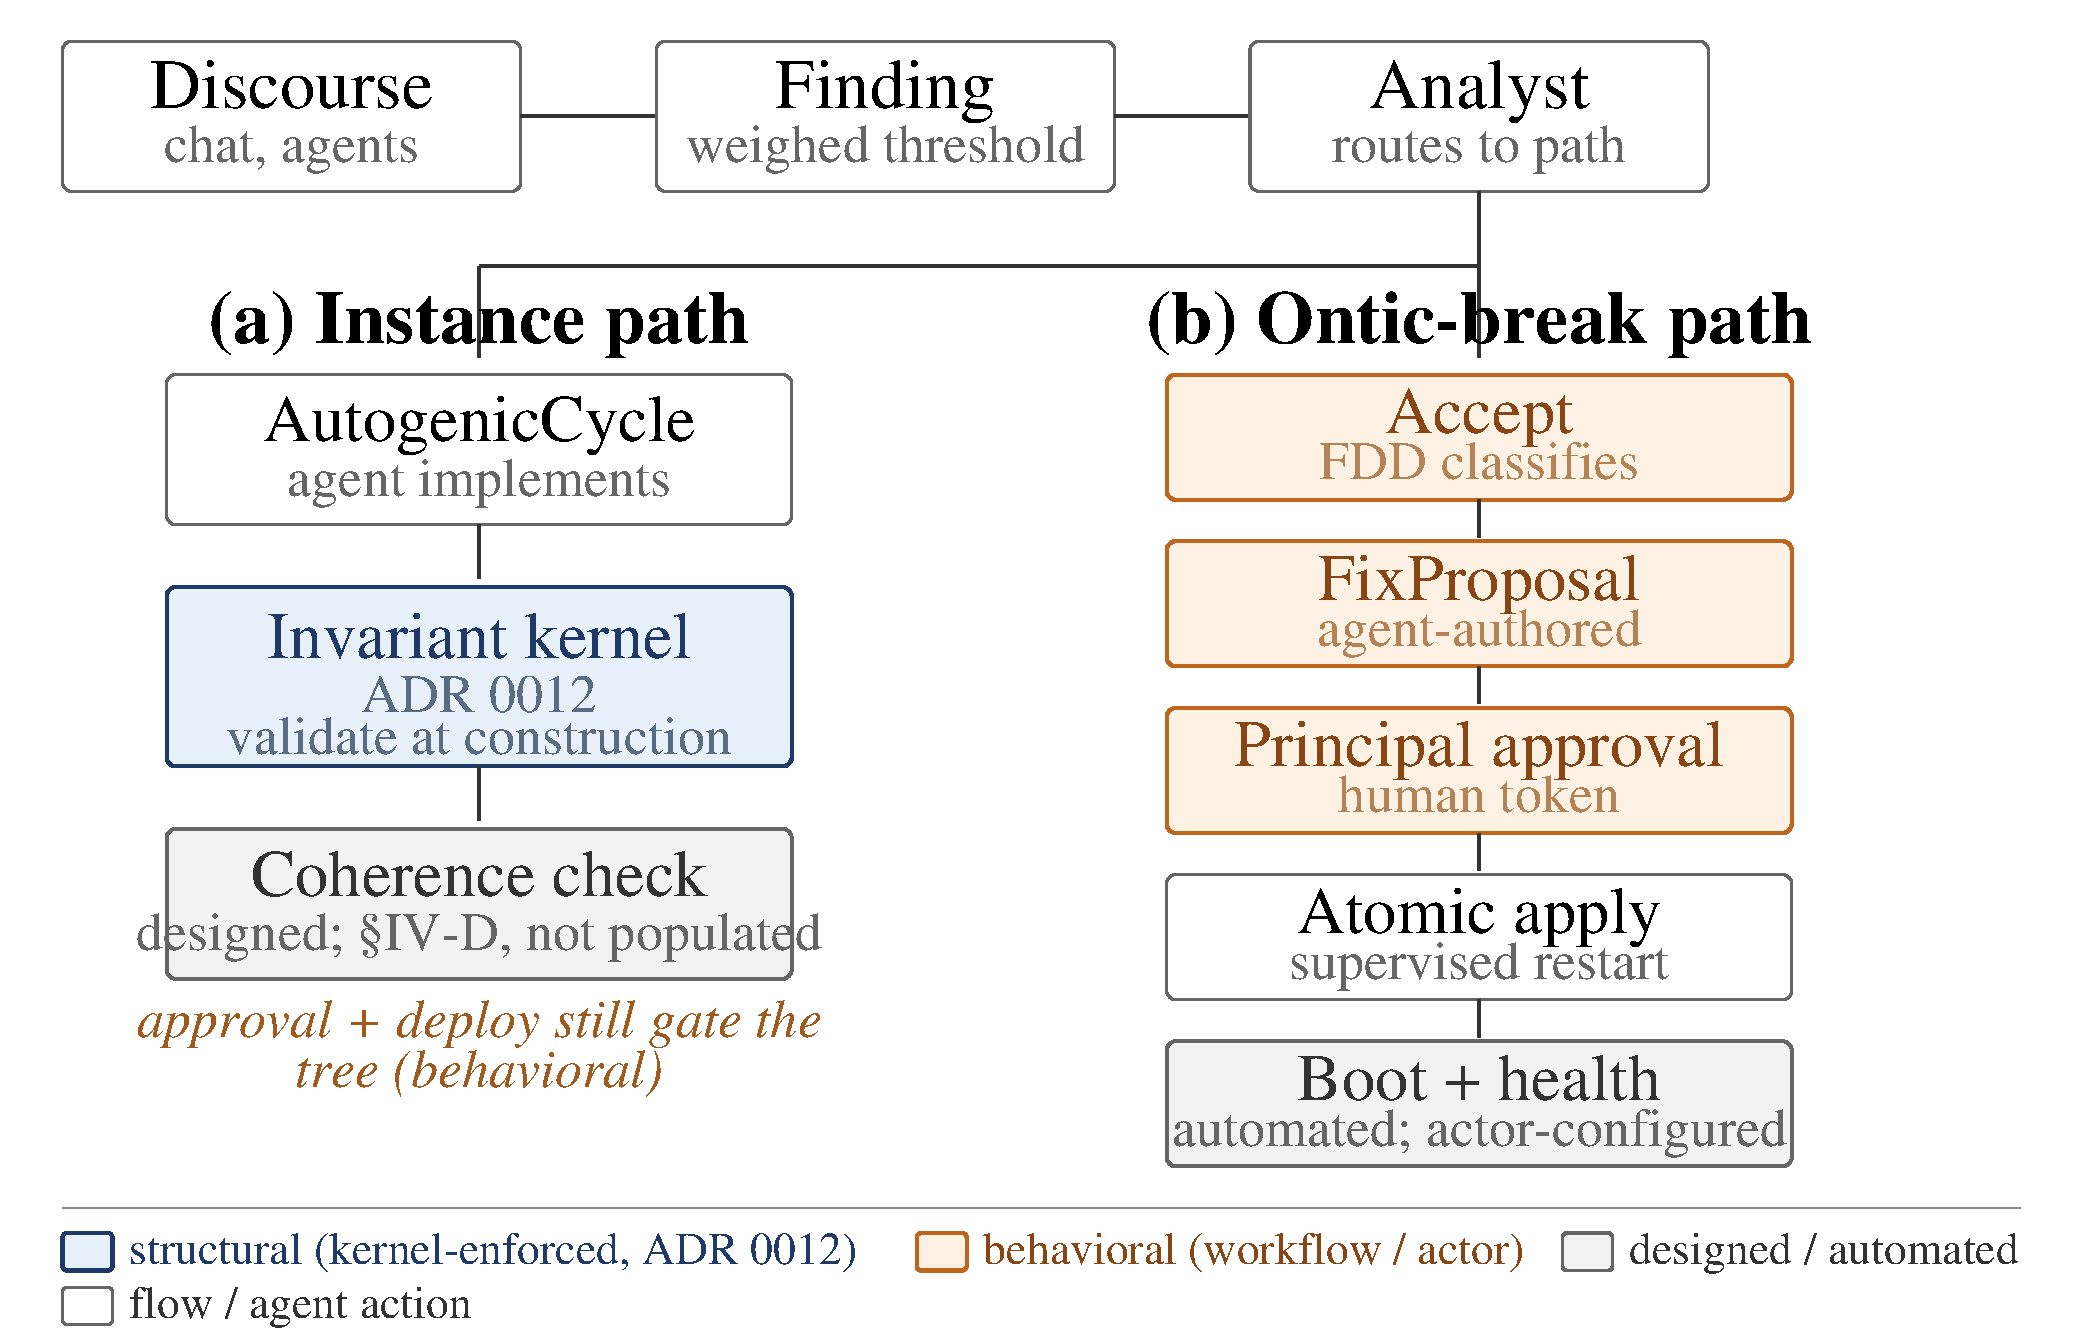
\includegraphics[width=\columnwidth]{figures/fig-mechanism}

\caption{Autogenic loop mechanism, as designed. Instance path: agent is autonomous at implementation; kernel validation (ADR 0012) is structural; the coherence check on completion is designed but was not populated over the reported window (§IV-D). Ontic-break path: agent-authored FixProposal, then human approval, atomic apply, and supervised restart (behavioral). Boot-and-health rollback is automated, actor-configured, not kernel-structural. Access-control gap (§IV-D): a sub-agent with repo write and \texttt{DATABASE\_URL} can bypass the workflow via \texttt{migrate}.}\label{fig:mechanism}

\end{figure}

\subsection{Reference architecture}\label{sec:reference}

The architecture is design-inspired by biological cognition; the
mapping below is analogy, not a functional-equivalence claim. Every
neural structure in the human brain accumulated across five hundred
million years of evolution. The build order fixes a dependency order: the oldest
structures handle the most fundamental problems and the newest the most
abstract. Ten mind components mirror ten neural structures: Cognitive Fabric --
Cerebral Cortex, Binding Engine -- Hippocampus, Evaluation Engine --
Amygdala, Selection Gate -- Basal Ganglia, Router -- Thalamus,
Prediction Engine -- Cerebellum, Conflict Monitor -- Anterior Cingulate,
Drive System -- VTA / dopamine circuits, Initiative Engine -- Pre-SMA,
Interconnect -- White Matter. The mapping supplies naming and rough
functional intent for each component; it is not a claim of
neuroscientific equivalence.

The architecture is \emph{autogenic}: its specification is embedded in the
running system. Six axioms follow (unity, emergence, identity,
embodiment, regeneration, determination). The system carries its own
specification and participates in its own construction.

Three body systems ground the ten mind components: Sensory (input),
Motor (output), and Interoceptive (internal state). The Interoceptive
system supplies the telemetry edge of the coherence triad
(§\ref{sec:triad}). Its runtime organs are the Anatomy classes
whose instances are the actual organs of the running body: \texttt{Process},
\texttt{Sensor}, \texttt{Effector}, \texttt{Store}, \texttt{Clock}, \texttt{Surface}.

\subsection{Ontology as declaration}\label{sec:ontology}

In Vega, the ontology is a \emph{catalog of classes}. One hundred and seven
declared classes at the time of writing, one hundred and five with an
explicit machine schema, each defined in \texttt{lib/proto/*.js} and registered
in a single manifest. The formal catalog was created on 6 July 2026.
The ontology structure during the reported run window (May-June 2026) was
carried informally as prompts, faculties, tool schemas, and migrations,
and the class-count trajectory through July and August is 40, then 68,
88, 94, and finally the live 107 at time of writing. The catalog is
organized under eight discipline packages named for the natural-science
lenses they correspond to: Anatomy, Physiology, Psychology, Ontogeny,
Sociology, Epistemics, Authorship, and Meta. Every entry carries an
identifier, a discipline, a build wave, a lifecycle state, a short
description, and a typed field list. The catalog is not a document. It
is registry data the agent reads about itself.

Each class carries a \emph{state} on the ladder \emph{planned} → \emph{procedural} →
\emph{instance}. A planned class is present in the catalog but does not yet
construct instances. A procedural class exists as behavior running in
ordinary code but not as a first-class object. An instance class
constructs and validates instances at runtime against its declared field
list. The ladder walks forward only. A class does not regress. Promotion
from one rung to the next is a discrete commit that ships a schema, a
class module, tests, and a state flip together (recipe in
Architecture Decision Record (ADR) 0014).

The disciplines carry vocabularies of their own. Epistemics holds
\texttt{epistemic\_nodes} with a nine-value \texttt{claim\_type} enum for Toulmin
argument structure \cite{toulmin1958}. Physiology holds \texttt{TelemetryEvent},
\texttt{Fault}, \texttt{ToolExecution}, each enum-locked. Ontogeny holds \texttt{Finding} with an enum-locked lifecycle \texttt{state} (\texttt{proposed}, \texttt{accepted}, \texttt{in\_progress}, \texttt{shipped}, \texttt{rejected}, \texttt{deferred}, \texttt{needs\_external\_dev}, \texttt{merged}). Sociology holds \texttt{Channel} with a
\texttt{visibility} enum (\emph{public}, \emph{private}, \emph{DM}). Meta holds the state
ladder as an enum (\emph{planned}, \emph{procedural}, \emph{instance}). Anatomy holds
the runtime organs: \texttt{Process}, \texttt{Sensor}, \texttt{Effector}, \texttt{Store}, \texttt{Clock},
\texttt{Surface}. Each is a class whose instances are the actual organs of
the running body.

Every one of these vocabularies is a closed enum enforced at the storage
layer. The database refuses an \texttt{INSERT} whose enum value is not on the
list. It does so before the application layer sees the row. For
concreteness: \texttt{entities.type} takes exactly nine values, locked by
migration \texttt{0096}. \texttt{epistemic\_nodes.claim\_type} takes exactly nine (the
Toulmin roles), locked by migration \texttt{0078}. There is no free-form
\emph{capability} category and no configuration field into which arbitrary
new kinds might quietly enter as instances. Widening an enum requires a
schema migration. Migrations are additive, forward-only, and
human-authored, enforced by \texttt{src/db.js}. Widening the catalog itself, by
adding a class, goes through the same discipline at a larger grain.

The catalog is neither a description of the code nor a description of a
domain outside the code. It is a set of declarations that prescribe what
the code and the agent can do next.
Fig. \ref{fig:mechanism} shows the loop's mechanism.

\subsection{The coherence triad}\label{sec:triad}

Under this condition, we read each part of the system through three
representations. The requirement declares what must be true. The code
implements it. The telemetry reports what happened. We call the
three-way relationship the \emph{coherence triad}. Verification is the
maintenance of coherence across its three edges where the substrate
carries all three.

Two edges are familiar. Requirement-code coherence is what a
specification matches against an implementation. Code-telemetry
coherence is what a test suite establishes: given a run, the observed
behavior matches the coded behavior. The third edge is the one the field
routinely leaves implicit. Requirement-telemetry coherence asks whether
what happens is what was asked for, independent of how the code got
there. Specification gaming \cite{krakovna2020,amodei2016,skalse2022} passes the tests by definition. It is
invisible on the code-telemetry edge and shows up only on the
requirement-telemetry edge. Naming all three edges is necessary but not sufficient: detection
also requires an encoded requirement, a suitable predicate, telemetry
that observes the relevant behavior, and an implemented monitor.
Within those conditions a coherence check can be exact: it
evaluates a declared constraint and returns yes or no, but exactness
of the predicate does not establish completeness of the encoding, the
telemetry, or the represented dependencies. A test suite samples
inputs.

\subsection{Two kinds of change}\label{sec:findings-taxonomy}

Two kinds of change follow from the declaration structure. The
distinction is precise.

An \emph{ontology instance} is a change the current catalog can already
express. A new \texttt{Message} on an existing \texttt{Channel} (Sociology). A new
\texttt{Finding} whose \texttt{state} reaches \texttt{shipped} through the enumerated transitions (Ontogeny).
A new epistemic node of \texttt{claim\_type} \emph{contention} (Epistemics). A new
\texttt{Draft} against an existing \texttt{Style} (Authorship). A new \texttt{TelemetryEvent}
row emitted by an existing \texttt{Sensor} (Anatomy). Each is a new row against
an existing instance class, drawing entirely from vocabularies the class
already permits. Instances are verified by the constraints declared
alongside the class. The database refuses inserts that violate them, and
the coherence triad then evaluates whether the new instance is
consistent with the existing requirement and telemetry. Instances constitute the ordinary growth of the system. Six roles
separate for a shipped Instance: origination, proposal, implementation
(agent); construction-time validation (invariant kernel, ADR 0012);
approval and deployment supervision (§\ref{sec:ontic-gate});
closure. The kernel is automated; the other roles retained human touch.

An \emph{ontic break} is a change the current catalog cannot express. Two
shapes occur. An \emph{enum widening} (a value outside a declared enum: a
claim kind, a \texttt{Channel.visibility}, a \texttt{Sensor} sub-type) requires a
migration. A \emph{class admission} (a requirement no existing class fits)
requires a new class walked from \emph{planned} to \emph{instance} per the
ADR-0014 recipe. The break is a requirement the agent cannot satisfy
with the vocabulary it has. The FDD lifecycle moves the Finding to
\texttt{needs\_external\_dev} for hand-off.

\subsection{The ontic-break gate}\label{sec:ontic-gate}

Naming the distinction gives us the safety gate. The gate is not a
single mechanism. It is a composite of three enforcement layers. At the
application-config layer, three ontology-bearing files carry an
\texttt{editable:\ false} flag that lifts them out of the sub-agent's writable
scope. At the workflow layer, the FDD lifecycle \cite{palmer2002} classifies affected
paths at accept, opens a FixProposal, and refuses to \texttt{apply} (or
\texttt{apply-and-deploy}) without a principal-review approval token
(\texttt{POST\ /api/coding/proposals/:id/approve} then \texttt{/apply} or
\texttt{/apply-and-deploy}). Accept may auto-dispatch generation; close does
not. Apply is atomic against the code tree; restart is supervised
(\texttt{scripts/vega-supervise.js} locally, Cloud Run revision hosted). At the
operator layer, the principal issues the approval token through a review
UI after inspecting the proposal. Together the three layers keep
sub-agents outside the loop that decides which schema files can be
edited and which ontic-break migrations can be applied.

We are careful about what this composite is and is not. Five guarantee
types separate. \emph{Structural} (kernel + enum locks refuse malformed
instances at construction). \emph{Behavioral} (FDD approval, deployment
supervision, auto-rollback, actor-driven). \emph{Access-control} is not
enforced: a sub-agent with repo write and \texttt{DATABASE\_URL} bypasses the
workflow by running \texttt{migrate} outside the coordinator. The workflow was configured to route ships through the gate. Records
verify FDD workflow entry for 35 of the 159 shipped, of which 15
reached verified or applied. The remaining 124 shipped Findings closed
without a proposal record and cannot be attributed to the gate from
records alone; absence of a record is not evidence of bypass, nor of
review outside the workflow.
The gate is workflow-and-config, not schema. That is the standard.
Schema conformance is not behavioral correctness: an ontology-compatible
instance can still change runtime behavior in ways the kernel does not
catch.

Failed apply-and-deploys auto-roll back on boot-and-health timeout or
reflection-verify mismatch (\texttt{stageRollback}); catalog rollback is
operator-only. Window: 1 auto-rollback (boot-and-health), 1 operator rollback, 3
proposals rejected before apply, 0 reflection-verify mismatches.

\section{Methods}\label{sec:methods}

\subsection{Vega and Boole}\label{sec:vega-boole}

Vega is a production platform whose primary surface is a chat interface
open to human users. Every message a user sends is captured as a claim
envelope in the epistemic layer described in
§\ref{sec:ontology}. Each envelope that reaches the \emph{weighed}
maturity state becomes a Finding: an addressable proposal for a change
to the system.

Boole is a coding agent hosted inside Vega. It reads the ontology,
receives Findings from the Vega surface, and orchestrates five
specialized sub-agents in the change-producing loop (Analyst, PM,
Designer, Architect, Telemetry; roles enumerated in
§\ref{sec:architecture}). Boole plus those five make six
in-loop; eighty-three infrastructure sub-agents sit outside, for
eighty-nine total. Full roster in the replication package.

\subsection{Architecture}\label{sec:architecture}

The architecture is a consequence of the framework, not a choice made
independently of it. The framework requires three things. First, an
ontology declaration the agent can read at query time. Second, a
coherence check across the three edges of the triad. Third, a routing
decision on every incoming Finding: instance path or hand-off. The six
in-loop sub-agents named in §\ref{sec:vega-boole} land each
requirement. Boole handles routing. The Analyst, PM, Designer, and
Architect handle class-level changes against declared constraints. The
Telemetry agent is designed to run coherence checks (§\ref{sec:measurement})
against the same database the dev team writes to. The infrastructure
sub-agents outside the loop produce no changes to code. Their presence
reflects that Vega is a running system, not a stripped-down harness.
Their absence from the change-producing loop matters for the attribution
claim in §\ref{sec:results}. Vega's six in-loop
agents sit in the range OpenHands \cite{openhands2025} uses. The larger
system total reflects representing infrastructure services as ontology
classes instantiated as sub-agents.

The invariant kernel (ADR 0012, \texttt{@mach33/core}) enforces class-schema
validity at construction; apply-and-deploy is the FDD lifecycle
(§\ref{sec:ontic-gate}).

\subsection{Development lifecycle}\label{sec:lifecycle}

The lifecycle begins with a step that has no counterpart in traditional
software development. \textbf{Self-discovery through epistemic weight produced
by agent-human discourse.} As exchanges accumulate on the Vega chat
surface, each is captured as a \texttt{ClaimEnvelope} and lifted into the
belief graph as an \texttt{EpistemicNode}. The node carries a maturity
(\emph{detected}, \emph{under\_evaluation}, \emph{weighed}, \emph{decayed}), a confidence,
and an options-style \texttt{greeks} pressure vector. The graph continuously
evaluates the weight of what the system believes, corroborates, and
contests. When a claim reaches the \emph{weighed} state and its pressure
vector crosses threshold, it surfaces as a \texttt{Finding}. A \texttt{Finding} is a
specific gap, contradiction, or opportunity the system has discovered
against the state of its own beliefs, not against an external
specification.

The Analyst decomposes each Finding into touched classes and instances.
\textbf{Best case}: every class and vocabulary value exists; the Designer
closes on the instance path through an \texttt{AutogenicCycle}. \textbf{Intermediate}:
a vocabulary value is missing, a narrower ontic break requiring an
enum-widening migration for human review. \textbf{Worst}: new classes must
walk from \emph{planned} through \emph{procedural} to \emph{instance} per ADR-0014,
accepted only if coherent. Every step is a \texttt{TransitionEvent} against
the Finding's \texttt{Lifecycle}.

\begin{figure}[!t]
\centering
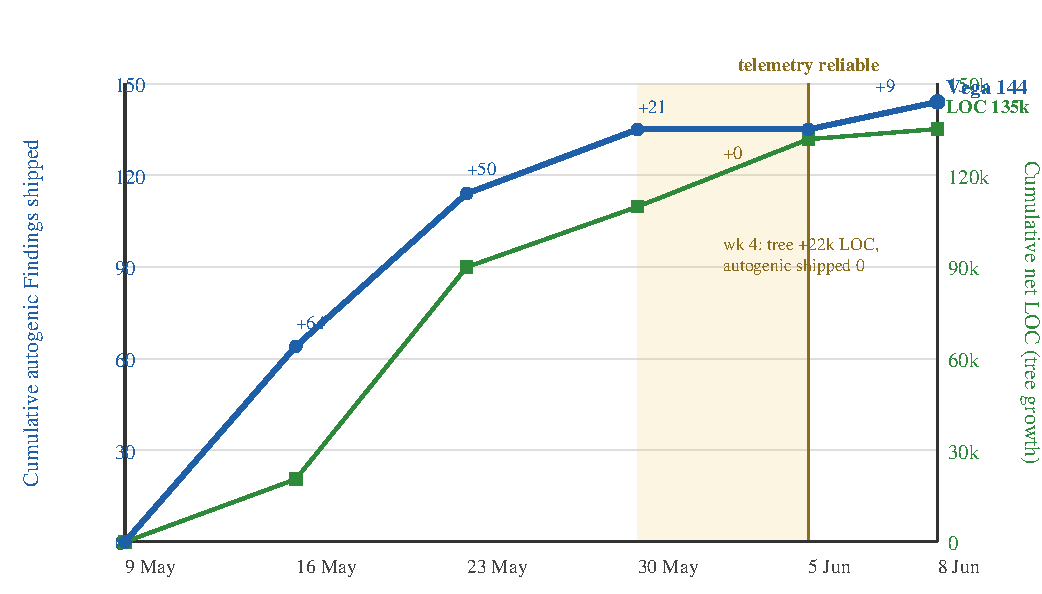
\includegraphics[width=0.85\columnwidth]{figures/fig-throughput}

\caption{Cumulative autogenic Findings shipped (left axis) and net LOC (right axis, tree, mixed authorship), 9 May -- 8 Jun 2026. Weekly Vega deltas 64/50/21/0/9; LOC 20.5k/69.4k/19.8k/22.1k/3.3k. Week 4 (30 May -- 5 Jun): 0 autogenic shipped while tree grew by 22k LOC; state-transition telemetry became reliable on 5 Jun (§IV-D). User-filed (15 shipped, weekly 9/2/2/0/2) reported in Table I. LOC pre-26 May are backfilled absolute counts; basis seams on 18 and 27 May are measurement changes, not deletions.}\label{fig:throughput}

\end{figure}

\subsection{The coding-agent loop}\label{sec:loop}

Inside every \texttt{AutogenicCycle} above, Boole runs an inner loop. The field
has converged on a common shape for it: reason-act-observe, repeated
until a task closes~\cite{react2023,sweagent2024,openhands2025}. The
agent inspects the state via grep or an embedding retriever,
reasons about what to do next, invokes a tool, observes the result, and
repeats. Termination is decided by the agent's own judgment against the
task specification.

Boole runs the same three-step loop with two substitutions dictated by
the ontology. \textbf{Reason} is a look-up, not a search. A query against the
class catalog returns exact class membership, constraint violations,
and transitive-closure blast radius within the declared ontology.
Runtime dependencies not represented in the ontology are not seen. The retrieval
approximation that binds a grep- or embedding-based reasoner
(§\ref{sec:intro}) is not there to bind Boole. In the design, \textbf{Observe} would consume both the tool result and a
coherence check on state-changing actions; a failing check would
prevent termination. Instrumentation for that event stream was not
populated during the reported window (§\ref{sec:threats});
coherence maintenance was not measured. Termination in the design is
decided against declared constraints of the touched classes, not the
agent's own judgment. This inverts the typical loop, which trusts the
agent's stopping criterion. Boole's design trusts the ontology's.

\subsection{Measurement}\label{sec:measurement}

The measurement instrumentation is thin by design. The
\texttt{M33-VEGA-INST-001} package writes numeric samples to an append-only
SHA-256-hashed JSONL chain across productivity, autogenic, and
code-quality categories; a \texttt{verifyChain()} endpoint reports
tamper-evidence. INST-001 (8 Aug 2026) and the formal catalog (6 July
2026) postdate the reported window; run-time governance was the
invariant kernel (ADR 0012) precursor and the FDD workflow as
configured. Numbers come from \texttt{code\_size\_snapshots} and
\texttt{self\_improvements}.

The coherence-triad check described in §\ref{sec:triad} is a
separate designed instrument. A \emph{coherence check} is the evaluation of a
declared constraint against the current state of the ontology and the
current telemetry stream. It is a boolean predicate the schema carries
as a \texttt{CHECK} or foreign-key constraint, or a query the ontology tables
can evaluate. The predicate returns \emph{holds} or \emph{fails} with a pointer to
the specific instance that produced the failure. Instrumentation for
that event stream is designed but not populated over the reported
window. Population is future work. §\ref{sec:threats}
discloses the gap.

The replication package is at \url{https://github.com/jbarseneau99/papers/tree/main/an-autogenic-agent}. It releases the ontology-catalog snapshot, the enum-locking schema migrations, the \texttt{M33-VEGA-INST-001} chain, the coherence-check design specification, and the paper source under the MIT License. Vega and Boole themselves remain proprietary.

\section{Results and Discussion}\label{sec:results}

\subsection{Throughput under the coherence framework}\label{sec:res-coherence}

The reported evidence is throughput under a designed coherence-triad
framework. The triad-holds hypothesis is not tested here; the
coherence-check event stream was designed but not populated. Throughput
(§\ref{sec:res-attribution}, Fig. \ref{fig:throughput}): 159 Findings shipped in the
reported window, of which 144 were autogenic (Vega-originated) and 15
user-filed. The FDD gate closed 15 of the 159. The coherence-check event stream that would produce
holds/fails counts over the same window is designed
(§\ref{sec:measurement}) but was not populated. Reporting
those counts is future work.

The shape is front-loaded: weekly Vega deltas 64, 50, 21, 0, 9; weeks
1--2 shipped 114 of the eventual 144. Week 4 shipped zero and
coincides with the state-transition-telemetry cutover; the plateau and
the source-shift are not separable. User weekly deltas were steady.
Net LOC totalled 135k (\textasciitilde4,506/day); LOC and Findings decouple in week
4 (Fig. \ref{fig:throughput}).

\subsection{Attribution}\label{sec:res-attribution}

The run produced 177 Findings (9 May -- 8 June 2026, 30 days), 159
shipped. 35 opened a \texttt{fix\_proposal}; 15 reached verified or applied.
The remaining 124 shipped without a proposal record. Separately, 117
of 159 are ontology-unclassified from records (Table
\ref{tab:findings-by-path}); the two counts are different
attributes. Intended policy (§\ref{sec:findings-taxonomy})
required human approval and supervised deployment on every ship; for
the 124 without a proposal record this is policy, not records-verified.
By \texttt{proposed\_by}: 144 agent (91\%), 15 user (9\%), 0 team.

Ship rate 89.8\% (159/177). Ontology split from records: 10/32/117
(Table I). 74\% lack the affected-file record; among the 15
verified/applied: 9 ontic-break, 5 instance, 1 unknown. Median close
8h 15m Vega / 6h 47m user; 5.3 shipped/day over the 30-day window.

\begin{table}[!t]
\centering

\caption{Findings by author, Vega FDD store, 9 May -- 8 June 2026 (30-day window). I / OB / Unk = ontology-classification split (Instance: no locked file, no migration, no \texttt{needs\_external\_dev} in closure diff; Ontic-break: migration, locked file, or \texttt{needs\_external\_dev}; Unknown: no affected-file record). S/d = shipped per day. 117 of 159 shipped are ontology-unclassified, 42 positively classified.}\label{tab:findings-by-path}
\small
\begin{tabular}{@{}lrrrrr@{}}
\hline
Author & Filed & Ship & I / OB / Unk & S/d & Median \\
\hline
Vega   & 161 & 144 & 4 / 28 / 112 & 4.8 & 8h 15m \\
User   &  16 &  15 & 6 /  4 /   5 & 0.5 & 6h 47m \\
Team   &   0 &   0 & 0 /  0 /   0 & 0.0 & --     \\
\hline
Total  & 177 & 159 & 10 / 32 / 117 & 5.3 & 8h 09m \\
\hline
\end{tabular}

\end{table}

\subsection{Specification-gaming detection}\label{sec:res-gaming}

Specification gaming, behavior that passes tests while failing the
requirement the tests were meant to protect, appears in a coherence
check as failure on the requirement-telemetry edge without a matching
code-telemetry failure, paired on the same transition id. This paper
describes the detector; validation is future work. Coverage is the
ontology's coverage: gaming that violates a declared constraint is
surfaced; gaming that satisfies every declared constraint while missing
an undeclared one is not.

\subsection{Threats to validity}\label{sec:threats}

Four threats attach. \emph{Single-platform, \(n=1\)}: coherence on Vega does
not entail coherence on a different system whose ontology is declared
differently; what generalizes is the shape of the argument, not the
numbers. \emph{Ontology-as-choice}: widening \texttt{entities.type} or replacing the
Toulmin \texttt{claim\_type} with a rhetorical structure would change what
counts as an instance versus an ontic break. The framework
distinguishes declared ontologies from latent ones, not good from bad. \emph{Two of three enforcement
mechanisms are behavioral, not structural}
(§\ref{sec:ontic-gate}): locked-region refusal and principal
review depend on an actor choosing to act. Only the storage-layer enum
lock is structural. A hostile agent routes around the softer gates. \emph{Instrumented by the observed
system}: the telemetry agent reads state from the same database it
writes to; the reads and writes are separated by role but a fully
independent observer would need to be hosted outside Vega.

State-transition telemetry began 5 June 2026. For 9 May--4 June,
Finding dates derive from \texttt{proposed\_at} and artifact metadata, not
logged transitions; closure dates in that stretch are lower-bound
estimates. Of the 159 shipped Findings, 35 opened a \texttt{fix\_proposal}; 15
reached verified or applied. Records do not identify the close path
for the 124 shipped without a proposal record. LOC and commits
(Fig. \ref{fig:throughput}) are surviving tree growth, mixed
authorship, not autogenic Findings. The
case study establishes operational feasibility and throughput under
the gate. A prospective matched evaluation is proposed future work: baseline agent, code-graph agent, and the ontology-based approach, held constant on model, tasks, tools, budget, and approval policy, measuring correct closure, missed violations, false alarms, regressions, human effort, and cost.

The coherence-check event stream (§\ref{sec:triad}) was
designed but not populated in the window. The empirical result is
throughput, not a holds/fails count. The ontic-break gate
(§\ref{sec:ontic-gate}) is workflow-and-config, not a
structural invariant of the schema: a sub-agent with repo write and
database credentials could bypass the workflow by running \texttt{migrate}
outside the coordinator.

\subsection{Related work}\label{sec:related}

Our position sits against five lines. \emph{Benchmark} (SWE-bench
\cite{swebench2024,swebench2026}, SWE-agent \cite{sweagent2024},
AutoCodeRover \cite{autocoderover2024}): agents closing bugs in code they
did not author; AutoCodeRover's AST is a partial structural break
with grep. \emph{Harness} (ReAct \cite{react2023}, OpenHands \cite{openhands2025},
Agarwal \cite{agarwal2026}, He \cite{he2026cursor}) improves the loop around
the model. \emph{Code-graph} (RepoGraph \cite{repograph2025}) makes the
repository graph explicit. These describe code; we prescribe with a
runtime ontology.

\emph{Runtime-model} (Models@run.time \cite{modelsatruntime2009}, Requirements
Reflection \cite{reqreflection2010}) established causally-connected
self-representations and runtime requirements. Our addition is the
instance-vs-ontic-break distinction and the composite gate. \emph{Self-evolving-agent} (SelfEvolve \cite{selfevolve2026}, SEAgent
\cite{seagent2025}, Gödel Agent \cite{godelagent2025}, Darwin Gödel
\cite{darwingodel2026}, Huxley-Gödel \cite{huxleygodel2026}): agent
modifies itself, unconstrained against a declared ontology.
Huxley-Gödel raises the self-improving bar to
capability-to-produce-better-agents; we measure throughput and do not
claim capability improvement. \emph{Ontology-of-agents} (AgentO
\cite{agento2026}) declares workflows over sixteen flat classes on
PROV-O and P-Plan; it describes an execution, ours prescribes.

\section{Conclusion}\label{sec:conclusion}

Mainstream coding agents leave runtime ontology latent and rediscover
it each session by search. This choice bounds what they can be
relied on to know. It explains the pattern of failures that has
accompanied their otherwise impressive progress. The assumption was
considered invariant until it wasn't.

The alternative is to declare the structure. The agent authors the code
it reads. The declaration prescribes. It does not describe. Verification
becomes coherence across the three edges of a triad that includes not
only the code and the tests but the requirement itself.

We ran the alternative on Vega for thirty consecutive days. Of the 177
Findings recorded (161 Vega-filed, 16 user-filed), 159 shipped. 35
opened a \texttt{fix\_proposal}; 15 reached verified or applied. Ship
classification: 10 confirmed instance, 32 confirmed ontic-break, 117
unclassified from records. Triad-hold is a designed check, not measured
in this window.

Whether the approach generalizes beyond the platform we built is open.
This paper names the choice, latent structure or declared structure, and
makes the second legible enough to try. The ontological declaration and
its ontic-break gate model a kernel-guarded, FDD-gated control loop for
self-improving agents. The inversion is the point.

\textbf{Use of Large Language Models.} Commercial APIs (Anthropic Claude,
xAI Grok) assisted with writing. Boole, the coding agent evaluated in
§\ref{sec:vega-boole}, is itself a commercial-LLM system
behind the human approve/apply gate of §\ref{sec:ontic-gate}.
No in-house models, no fine-tuning. Vega and Boole are internally
deployed, not public inference. Counts in
§\ref{sec:res-attribution} were recomputed from production
\texttt{self\_improvements}.


% MD-BODY-END — end of the MD-editable region.
% ============================================================================

% ============================================================================
%  APPENDICES
% ============================================================================
% Appendices moved out for the 6-page limit. All three appendix sections
% (Sub-agent roster + table, Ontology schema, Reproducibility bulleted
% inventory) live in the replication-package companion doc; the body
% carries a one-line pointer at each site of use. The Sub-agent roster
% count is stated inline in Methods (§Vega and Boole).
%
% Companion doc: \TODO{tech-report-url}

% ============================================================================
%  REFERENCES
% ============================================================================
% refs.bib lives alongside paper.tex now (seeded from the archived AgenticDev
% draft during the repo reorg; per-paper bib is the idiomatic layout).
\bibliographystyle{IEEEtran}
\bibliography{refs}

\end{document}
